\subsection{Aufbau} \label{cap:methoden_aufbau}


Der Aufbau setzt sich aus sich aus folgenden Elementen zusammen: 
\begin{itemize}
\item Elektromagnet		
\item C-Schienen	
\item Aluminumscheibe	
\item ETG-100 Scheibe
\item Gestell für den Elektromagnet
\end{itemize}

Die ETG-100 Scheibe wird als erstes an das Schwungrad montiert. Auf die ETG-100 Platte folgt direkt die Aluminiumscheibe. Diese Armatur wurde starr verschraubt. 
Auf die Stand-Eisenträger des Spinning Wheels wurde das Gestell für den Elektromagneten fixiert. Auf dieses Gestell wurden die zwei C-Schienen angeschgraubt. Auf den C-Schienen wurde der Elektromagnet montiert. Dieser U-förmige Magnet schaut anschliessend mit den Pol-Austritten genau auf die Aluminiumscheibe zu. Die Wicklungen wurden über die Zylinder des Elektromagneten angebracht (Abbildung \ref{fig:gesamtaufbau}).

\begin{figure}[ht]
  \begin{center}
    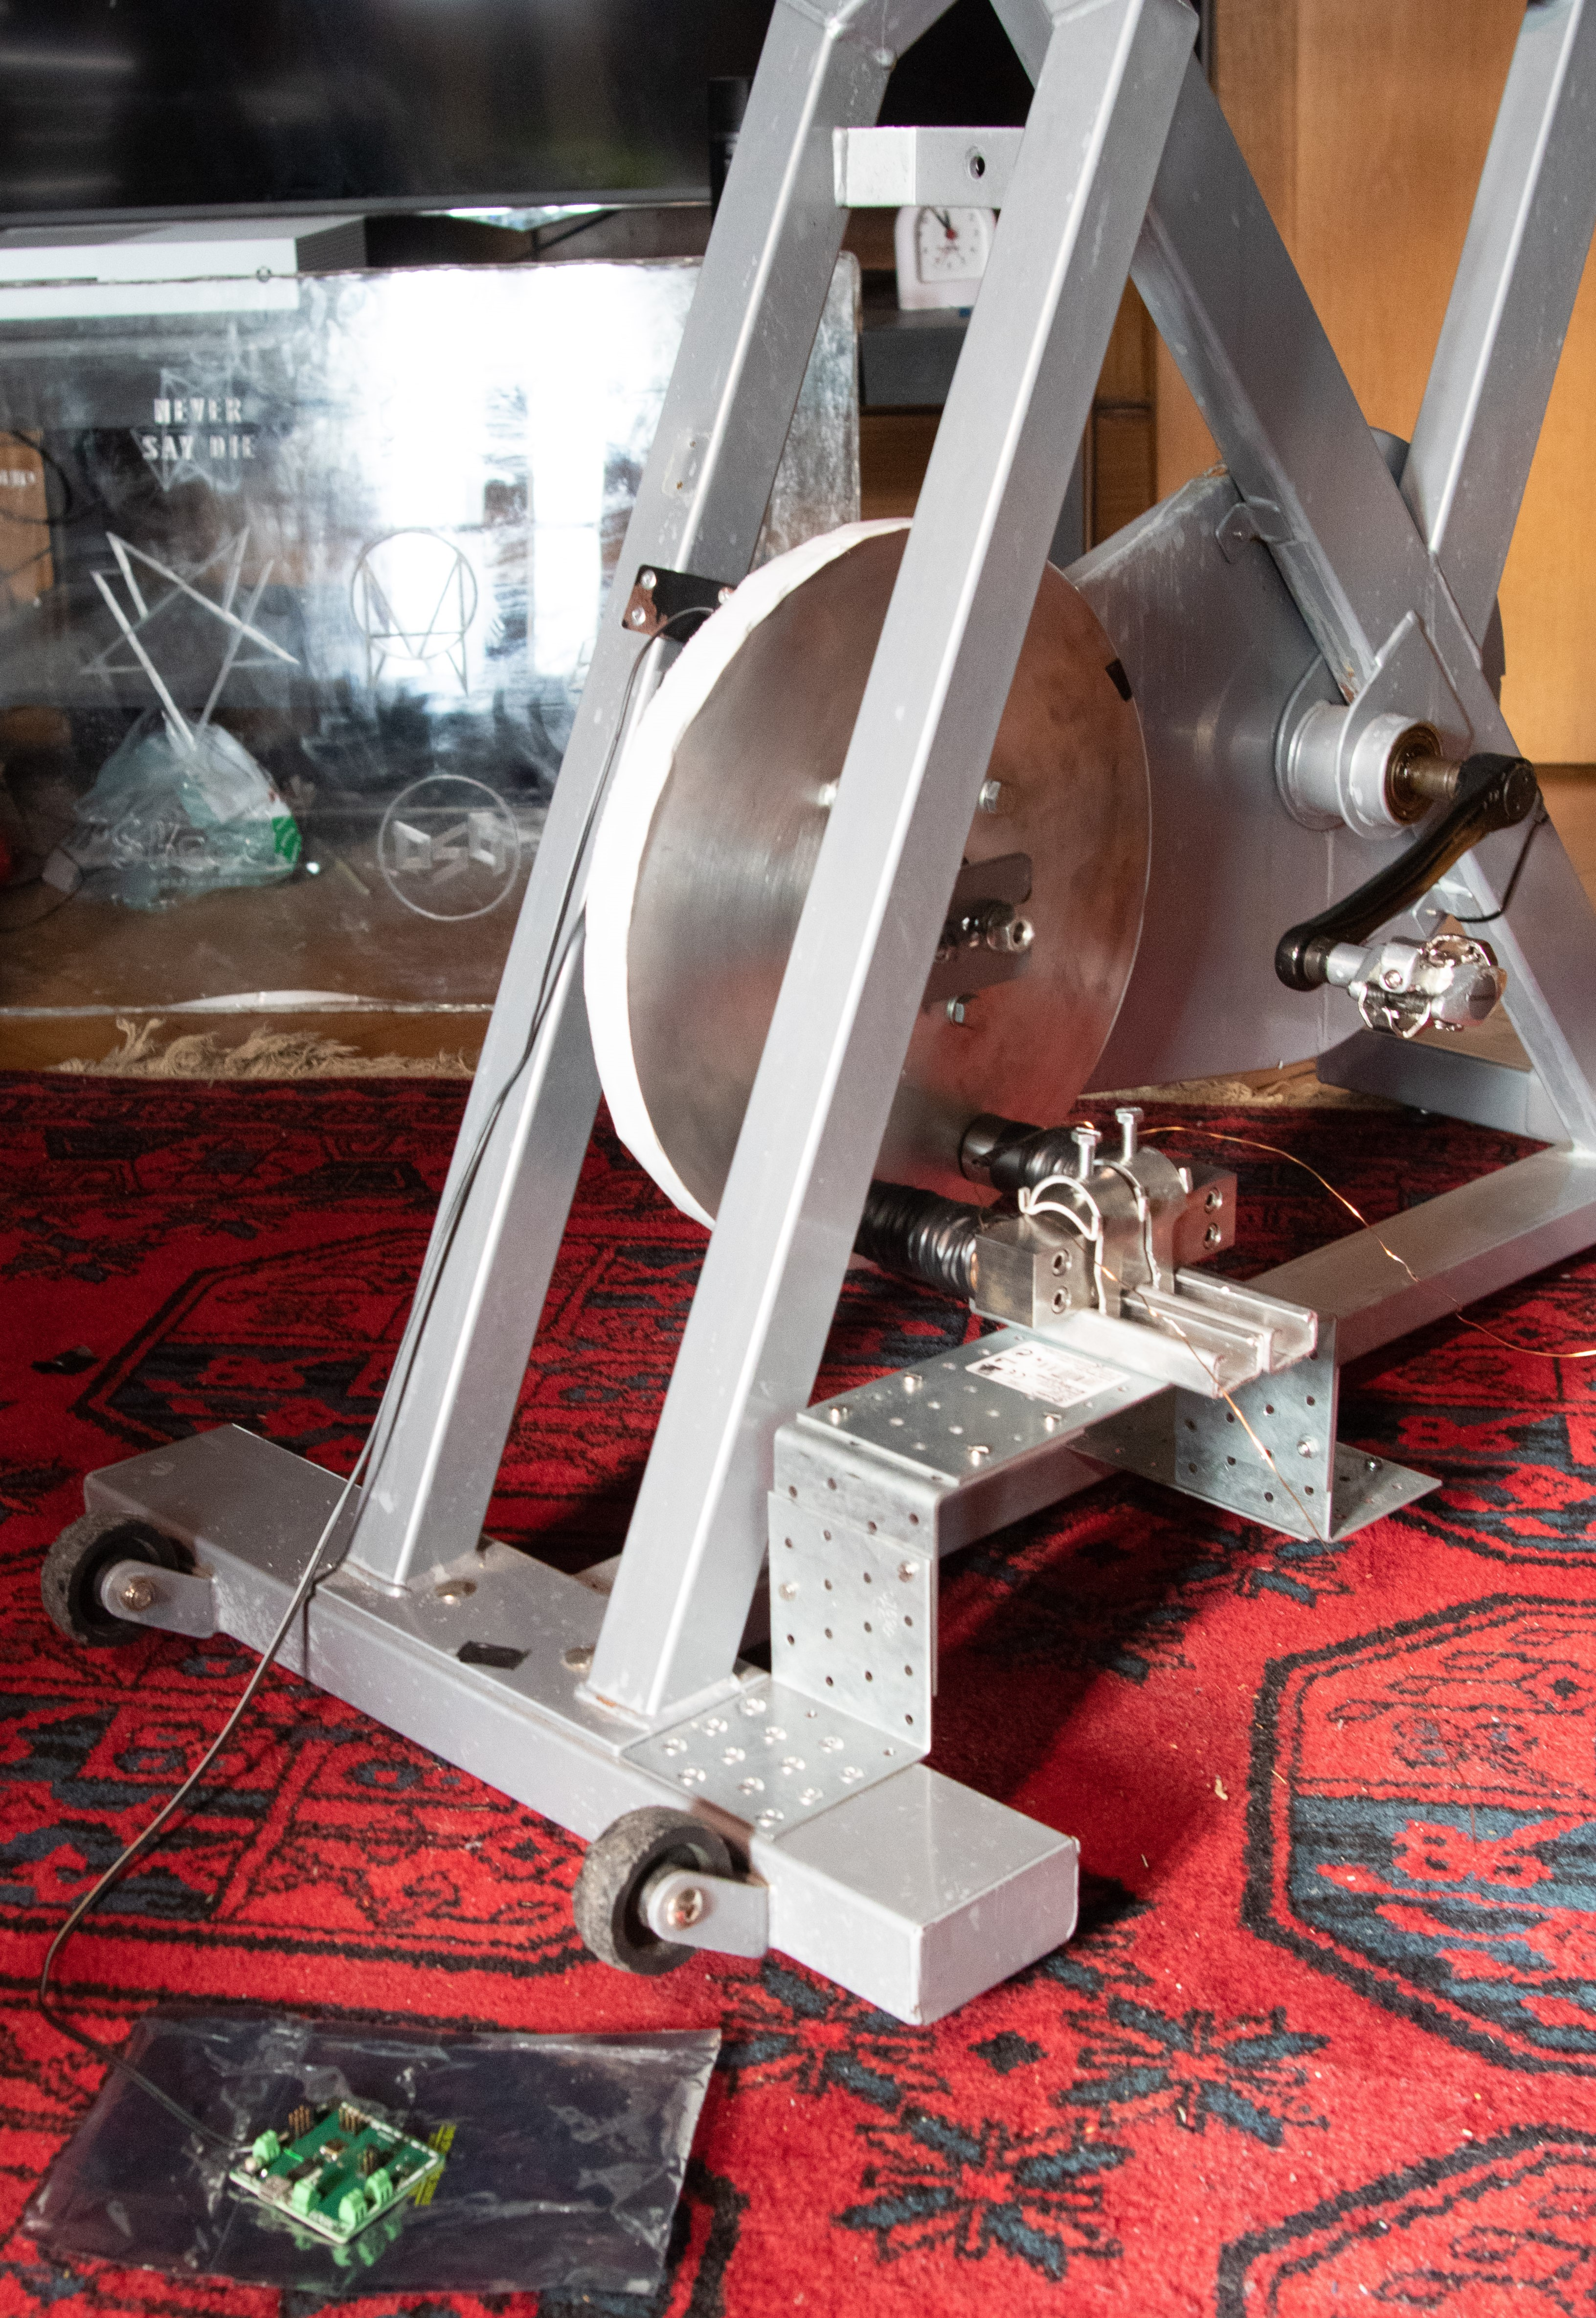
\includegraphics[height=10cm]{assets/images/aufbau/aufbau_magnet}
  \end{center}
  \vspace{-3ex}
  \caption{Gesamtaufbau}
  \label{fig:gesamtaufbau}
\end{figure}